
%{{第十回}}{第十回}}

\chapter{金寡妇贪利权受辱\hspace{.5em}张太医论病细穷源}

{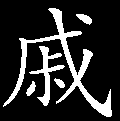
\includegraphics[width=3mm]{../Images/00005}  \kaishu  新样幻情欲收拾,可卿从此世无缘。和肝益气浑闲事,谁识今朝寻病源?}

话说金荣因人多势众,又兼贾瑞勒令,赔了不是,给秦钟磕了头,宝玉方才不吵闹了。大家散了学,金荣回到家中,越想越气,说:``秦钟不过是贾蓉的小舅子,又不是贾家的子孙,附学读书,也不过和我一样。他因仗着宝玉和他好,他就目中无人。他既是这样,就该行些正经事,人也没的说。他素日又和宝玉鬼鬼祟祟的,只当我们都是瞎子,看不见。今日他又去勾搭人,偏偏的撞在我眼里。{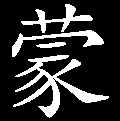
\includegraphics[width=3mm]{../Images/00006}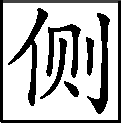
\includegraphics[width=3mm]{../Images/00011}\footnotesize \kaishu 偏是鬼鬼祟祟者,多以为人不见其行,不知其心。}就是闹出事来,我还怕什么不成?''

他母亲胡氏听见他咕咕嘟嘟的说,因问道:``你又要增什么闲事?好容易{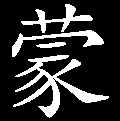
\includegraphics[width=3mm]{../Images/00006}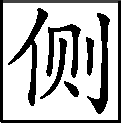
\includegraphics[width=3mm]{../Images/00011}\footnotesize \kaishu ``好容易''三字,写尽天下迎逢要便宜苦恼。}我望你姑妈说了,你姑妈千方百计的才向他们西府里的琏二奶奶跟前说了,你才得了这个念书的地方。若不是仗着人家,咱们家里还有力量请的起先生?况且人家学里,茶也是现成的,饭也是现成的。你这二年在那里念书,家里也省好大的嚼用呢。省出来的,你又爱穿件鲜明衣服。再者,不是因你在那里念书,你就认得什么薛大爷了?那薛大爷一年不给不给,这二年也帮了咱们有七八十两银子。{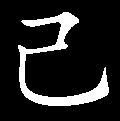
\includegraphics[width=3mm]{../Images/00003}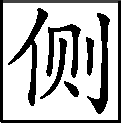
\includegraphics[width=3mm]{../Images/00011}\footnotesize \kaishu 因何无故给许多银子?金母亦当细思之。}\href{../Text/part0014_split_000.html\#lnkback_1_a}{\textsuperscript{①}}{ 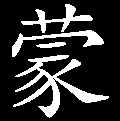
\includegraphics[width=3mm]{../Images/00006}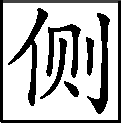
\includegraphics[width=3mm]{../Images/00011}\footnotesize \kaishu 可怜!妇人爱子,每每如此。自知所得者多,而不知所失者大,可胜叹者!}你如今要闹出了这个学房,再要找这么个地方,我告诉你说罢,比登天还难呢!{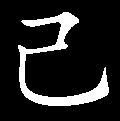
\includegraphics[width=3mm]{../Images/00003}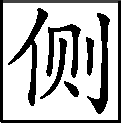
\includegraphics[width=3mm]{../Images/00011}\footnotesize \kaishu 如此弄银,若有金荣在,亦可得。}你给我老老实实的顽一会子睡你的觉去,好多着呢。''于是金荣忍气吞声,不多一时他自去睡了。次日仍旧上学去了。不在话下。

且说他姑娘,原聘给的是贾家玉字辈的嫡派,名唤贾璜。但其族人那里皆能像宁荣二府的富势,原不用细说。这贾璜夫妻守着些小的产业,又时常到宁荣二府里去请请安,又会奉承凤姐儿并尤氏,所以凤姐儿尤氏也时常资助资助他,{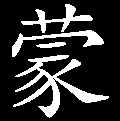
\includegraphics[width=3mm]{../Images/00006}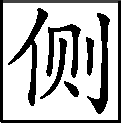
\includegraphics[width=3mm]{../Images/00011}\footnotesize \kaishu 原来根由如此,大与秦钟不同。}方能如此度日。今日正遇天气晴明,又值家中无事,遂带了一个婆子,坐上车,来家里走走,瞧瞧寡嫂并侄儿。

闲话之间,金荣的母亲偏提起昨日贾家学房里的那事,从头至尾,一五一十都向他小姑子说了。这璜大奶奶不听则已,听了,一时怒从心上起,说道:``这秦钟小崽子是贾门的亲戚,难道荣儿不是贾门的亲戚?{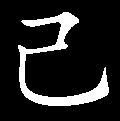
\includegraphics[width=3mm]{../Images/00003}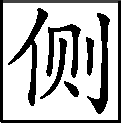
\includegraphics[width=3mm]{../Images/00011}\footnotesize \kaishu 这``贾门的亲戚''比那``贾门的亲戚''!}人都别忒势利了,况且都作的是什么有脸的好事!就是宝玉,也犯不上向着他到这个样。等我去到东府瞧瞧我们珍大奶奶,再向秦钟他姐姐说说,叫他评评这个理。''{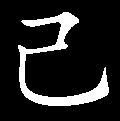
\includegraphics[width=3mm]{../Images/00003}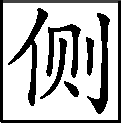
\includegraphics[width=3mm]{../Images/00011}\footnotesize \kaishu 未必能如此说。 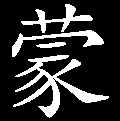
\includegraphics[width=3mm]{../Images/00006}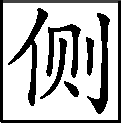
\includegraphics[width=3mm]{../Images/00011}\footnotesize \kaishu 狗仗人势者,开口便有多少必胜之谈,事要三思,免劳后悔。}这金荣的母亲听了这话,急的了不得,忙说道:``这都是我的嘴快,告诉了姑奶奶了,求姑奶奶别去,别管他们谁是谁非。{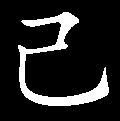
\includegraphics[width=3mm]{../Images/00003}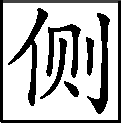
\includegraphics[width=3mm]{../Images/00011}\footnotesize \kaishu 不论谁是谁非,有钱就可矣。 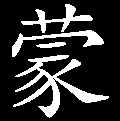
\includegraphics[width=3mm]{../Images/00006}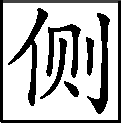
\includegraphics[width=3mm]{../Images/00011}\footnotesize \kaishu 胡氏可谓善哉!}倘或闹起来,怎么在那里站得住。若是站不住,家里不但不能请先生,反倒在他身上添出许多嚼用来呢。''璜大奶奶听了,说道:``那里管得许多,你等我说了,看是怎么样!''也不容他嫂子劝,一面叫老婆子瞧了车,就坐上往宁府里来。{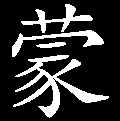
\includegraphics[width=3mm]{../Images/00006}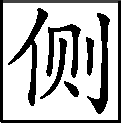
\includegraphics[width=3mm]{../Images/00011}\footnotesize \kaishu 何等气派,何等声势,真有射石饮羽之力,动天摇地,如项羽喑咤。}

到了宁府,进了车门,到了东边小角门前下了车,进去见了贾珍之妻尤氏。也未敢气高,殷殷勤勤叙过寒温,说了些闲话,方问道:{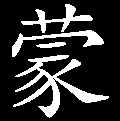
\includegraphics[width=3mm]{../Images/00006}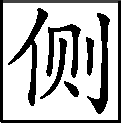
\includegraphics[width=3mm]{../Images/00011}\footnotesize \kaishu 何故兴致索然?}``今日怎么没见蓉大奶奶?''{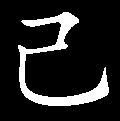
\includegraphics[width=3mm]{../Images/00003}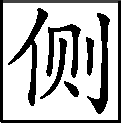
\includegraphics[width=3mm]{../Images/00011}\footnotesize \kaishu 何不叫``秦钟的姐姐''?}尤氏说道:``他这些日子不知怎么着,经期有两个多月没来。叫大夫瞧了,又说并不是喜。那两日,到了下半天就懒待动,话也懒待说,眼神也发眩。我说他:`你且不必拘礼,早晚不必照例上来,你就好生养养罢。就是有亲戚一家儿来,有我呢。就有长辈们怪你,等我替你告诉。'连蓉哥我都嘱咐了,我说:`你不许累他,不许招他生气,叫他静静的养养就好了。{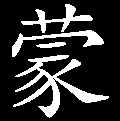
\includegraphics[width=3mm]{../Images/00006}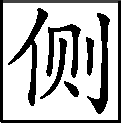
\includegraphics[width=3mm]{../Images/00011}\footnotesize \kaishu 只一丝不露。}他要想什么吃,只管到我这里取来。倘或我这里没有,只管望你琏二婶子那里要去。倘或他有个好和歹,你再要娶这么一个媳妇,这么个模样儿,这么个性情的人儿,打着灯笼也没地方找去。'{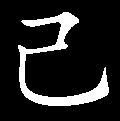
\includegraphics[width=3mm]{../Images/00003}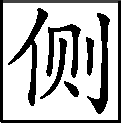
\includegraphics[width=3mm]{../Images/00011}\footnotesize \kaishu 还有这么个好小舅子。}他这为人行事,那个亲戚,那个一家的长辈不喜欢他?所以我这两日好不烦心,焦的我了不得。偏偏今日早晨他兄弟来瞧他,谁知那小孩子家不知好歹,看见他姐姐身上不大爽快,就有事也不当告诉他,别说是这么一点子小事,就是你受了一万分的委曲,也不该向他说才是。谁知他们昨儿学房里打架,不知是那里附学来的一个人欺侮了他了。{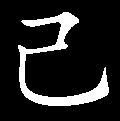
\includegraphics[width=3mm]{../Images/00003}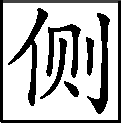
\includegraphics[width=3mm]{../Images/00011}\footnotesize \kaishu 眼前竟像不知者。 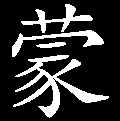
\includegraphics[width=3mm]{../Images/00006}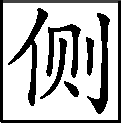
\includegraphics[width=3mm]{../Images/00011}\footnotesize \kaishu 文笔之妙,妙至于此。本是璜大奶奶不忿来告,又偏从尤氏口中先出,确是秦钟之语,且是情理必然,形势逼近。孙悟空七十二变,未有如此灵巧活跳。}里头还有些不干不净的话,都告诉了他姐姐。婶子,你是知道那媳妇的:虽则见了人有说有笑,会行事儿,他可心细,心又重,不拘听见个什么话儿,都要度量个三日五夜才罢。这病就是打这个秉性上头思虑出来的。今儿听见有人欺负了他兄弟,又是恼,又是气。恼的是那群混帐狐朋狗友的扯是搬非、调三惑四那些人;气的是他兄弟不学好,不上心念书,以致如此学里吵闹。他听了这事,今日索性连早饭也没吃。我听见了,我方到他那边安慰了他一会子,又劝解了他兄弟一会子。我叫他兄弟到那府里去找宝玉去了,我才看着他吃了半盏燕窝汤,我才过来了。婶子,你说我心焦不心焦?{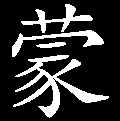
\includegraphics[width=3mm]{../Images/00006}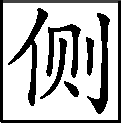
\includegraphics[width=3mm]{../Images/00011}\footnotesize \kaishu 这会子金氏听了这话,心里当如何料理?实在令人悔杀从前高兴。天下事不得不预为三思,先为防渐。}况且如今又没个好大夫,我想到他这病上,我心里倒像针扎似的。你们知道有什么好大夫没有?''{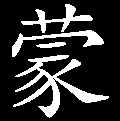
\includegraphics[width=3mm]{../Images/00006}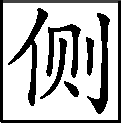
\includegraphics[width=3mm]{../Images/00011}\footnotesize \kaishu 作无意相问语,是逼近一分,非有此一句,则金氏犹不免当为分诉。一逼之下,实无可赘之词。}

金氏听了这半日话,把方才在他嫂子家的那一团要向秦氏理论的盛气,早吓的都丢在爪洼国去了。{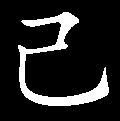
\includegraphics[width=3mm]{../Images/00003}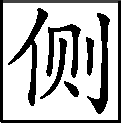
\includegraphics[width=3mm]{../Images/00011}\footnotesize \kaishu 又何必为金母着急。}听见尤氏问他有知道好大夫的话,连忙答道:``我们这么听着,实在也没见人说有个好大夫。如今听起大奶奶这个来,定不得还是喜呢。嫂子倒别教人混治。倘或认错了,这可是了不得的。''尤氏道:``可不是呢。''正是说话间,贾珍从外进来,见了金氏,便向尤氏问道:``这不是璜大奶奶么?''金氏向前给贾珍请了安。贾珍向尤氏说道:``让这大妹妹吃了饭去。''贾珍说着话,就过那屋里去了。金氏此来,原要向秦氏说说秦钟欺负了他侄儿的事,听见秦氏有病,不但不能说,亦且不敢提了。况且贾珍尤氏又待的很好,反转怒为喜,又说了一会子话儿,方家去了。{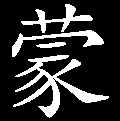
\includegraphics[width=3mm]{../Images/00006}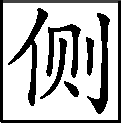
\includegraphics[width=3mm]{../Images/00011}\footnotesize \kaishu 金氏何面目再见江东父老?然而如金氏者,世不乏其人。}

金氏去后,贾珍方过来坐下,问尤氏道:``今日他来,有什么说的事情么?''尤氏答道:``倒没说什么。一进来的时候,脸上倒像有些着了恼的气色似的,及说了半天话,又提起媳妇这病,他倒渐渐的气色平定了。你又叫让他吃饭,他听见媳妇这么病,也不好意思只管坐着,又说了几句闲话儿就去了,倒没求什么事。如今且说媳妇这病,你到那里寻一个好大夫来与他瞧瞧要紧,可别耽误了。现今咱们家走的这群大夫,那里要得?{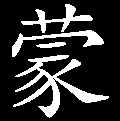
\includegraphics[width=3mm]{../Images/00006}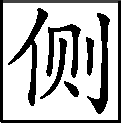
\includegraphics[width=3mm]{../Images/00011}\footnotesize \kaishu 医毒。非止近世,从古有之。}一个个都是听着人的口气儿,人怎么说,他也添几句文话儿说一遍。可倒殷勤的很,三四个人一日轮流着倒有四五遍来看脉。他们大家商量着立个方子,吃了也不见效,倒弄得一日换四五遍衣裳,坐起来见大夫,其实于病人无益。''贾珍说道:``可是。这孩子也糊涂,何必脱脱换换的,倘再着了凉,更添一层病,那还了得。衣裳任凭是什么好的,可又值什么,孩子的身子要紧,就是一天穿一套新的,也不值什么。我正进来要告诉你:方才冯紫英来看我,他见我有些抑郁之色,问我是怎么了。我才告诉他说,媳妇忽然身子有好大的不爽快,因为不得个好太医,断不透是喜是病,又不知有妨碍无妨碍,所以我这两日心里着实着急。冯紫英因说起他有一个幼时从学的先生,姓张名友士,学问最渊博的,更兼医理极深,且能断人的生死。{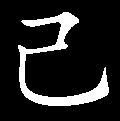
\includegraphics[width=3mm]{../Images/00003}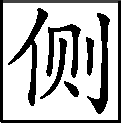
\includegraphics[width=3mm]{../Images/00011}\footnotesize \kaishu 未必能如此。 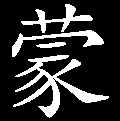
\includegraphics[width=3mm]{../Images/00006}\includegraphics[width=3mm]{../Images/00011}\footnotesize \kaishu 举荐人的通套,多是如此说。}今年是上京给他儿子来捐官,现在他家住着呢。这么看来,竟是合该媳妇的病在他手里除灾亦未可知。我即刻差人拿我的名帖请去了。{\includegraphics[width=3mm]{../Images/00006}\includegraphics[width=3mm]{../Images/00011}\footnotesize \kaishu 父母之心,昊天罔极。}今日倘或天晚了不能来,明日想必一定来。况且冯紫英又即刻回家亲自去求他,务必叫他来瞧瞧。等这个张先生来瞧了再说罢。''

尤氏听了,心中甚喜,因说道:``后日是太爷的寿日,到底怎么办?''贾珍说道:``我方才到了太爷那里去请安,兼请太爷来家来受一受一家子的礼。太爷因说道:`我是清净惯了的,我不愿意往你们那是非场中去闹去。你们必定说是我的生日,要叫我去受众人些头,莫过你把我从前注的《阴骘文》给我令人好好的写出来刻了,比叫我无故受众人的头还强百倍呢。倘或后日这两日一家子要来,你就在家里好好的款待他们就是了。也不必给我送什么东西来,连你后日也不必来,你要心中不安,你今日就给我磕了头去。{\includegraphics[width=3mm]{../Images/00006}\includegraphics[width=3mm]{../Images/00011}\footnotesize \kaishu 将写可卿之好事多虑。至于天生之文中,转出好清静之一番议论,清新醒目,立见不凡。}倘或后日你要来,又跟随多少人来闹我,我必和你不依。'如此说了又说,后日我是再不敢去的了。且叫来升来,吩咐他预备两日的筵席。''尤氏因叫人叫了贾蓉来:``吩咐来升照旧例预备两日的筵席,要丰丰富富的。你再亲自到西府里去请老太太、大太太、二太太和你琏二婶子来逛逛。你父亲今日又听见一个好大夫,业已打发人请去了,想必明日必来。你可将他这些日子的病症细细的告诉他。''

贾蓉一一的答应着出去了。正遇着方才去冯紫英家请那先生的小子回来了,因回道:``奴才方才到了冯大爷家,拿了老爷的名帖请那先生去。那先生说道:`方才这里大爷也向我说了。但是今日拜了一天的客,才回到家,此时精神实在不能支持,就是去到府上也不能看脉。'他说等调息一夜,明日务必到府。{\includegraphics[width=3mm]{../Images/00006}\includegraphics[width=3mm]{../Images/00011}\footnotesize \kaishu 医生多是推三阻四,拿腔作调。}他又说,他`医学浅薄,本不敢当此重荐,因我们冯大爷和府上的大人既已如此说了,又不得不去,你先替我回明大人就是了。大人的名帖实不敢当。'仍叫奴才拿回来了。哥儿替奴才回一声儿罢。''贾蓉转身复进去,回了贾珍尤氏的话,方出来叫了来升来,吩咐他``预备两日的筵席''的话。来升听毕,自去照例料理。不在话下。

且说次日午间,人回道:``请的那张先生来了。''贾珍遂延入大厅坐下。茶毕,方开言道:``昨承冯大爷示知老先生人品学问,又兼深通医学,小弟不胜钦仰之至。''张先生道:``晚生粗鄙下士,本知见浅陋,昨因冯大爷示知,大人家第谦恭下士,又承呼唤,敢不奉命。但毫无实学,倍增颜汗。''贾珍道:``先生何必过谦。就请先生进去看看儿妇,仰仗高明,以释下怀。''于是,贾蓉同了进去。到了贾蓉居室,见了秦氏,向贾蓉说道:``这就是尊夫人了?''贾蓉道:``正是。请先生坐下,让我把贱内的病症说一说再看脉如何?''那先生道:``依小弟的意思,竟先看过脉再说的为是。我是初造尊府的,本也不晓得什么,但是我们冯大爷务必叫小弟过来看看,小弟所以不得不来。如今看了脉息,看小弟说的是不是,再将这些日子的病势讲一讲,大家斟酌一个方儿,可用不可用,那时大爷再定夺。''贾蓉道:``先生实在高明,如今恨相见之晚。就请先生看一看脉息,可治不可治,以便使家父母放心。''于是家下媳妇们捧过大迎枕来,一面给秦氏拉着袖口,露出脉来。先生方伸手按在右手脉上,调息了至数,宁神细诊了有半刻的工夫,方换过左手,亦复如是。诊毕脉息,说道:``我们外边坐罢。''

贾蓉于是同先生到外间房里床上坐下,一个婆子端了茶来。贾蓉道:``先生请茶。''于是陪先生吃了茶,遂问道:``先生看这脉息,还治得治不得?''先生道:``看得尊夫人这脉息:左寸沉数,左关沉伏,右寸细而无力,右关需而无神。其左寸沉数者,乃心气虚而生火;左关沉伏者,乃肝家气滞血亏。右寸细而无力者,乃肺经气分太虚;右关需而无神者,乃脾土被肝木克制。心气虚而生火者,应现经期不调,夜间不寐。肝家血亏气滞者,必然肋下疼胀,月信过期,心中发热。肺经气分太虚者,头目不时眩晕,寅卯间必然自汗,如坐舟中。脾土被肝木克制者,必然不思饮食,精神倦怠,四肢酸软。据我看这脉息,应当有这些症候才对。或以这个脉为喜脉,则小弟不敢从其教也。''旁边一个贴身伏侍的婆子道:``何尝不是这样呢。真正先生说的如神,倒不用我们告诉了。如今我们家里现有好几位太医老爷瞧着呢,都不能的当真切的这么说。有一位说是喜,有一位说是病,这位说不相干,那位说怕冬至,总没有个准话儿。求老爷明白指示指示。''

那先生笑{\includegraphics[width=3mm]{../Images/00006}\includegraphics[width=3mm]{../Images/00011}\footnotesize \kaishu 说是了,不觉笑,描出神情跳跃,如见其人。}道:``大奶奶这个症候,可是那众位耽搁了。要在初次行经的日期就用药治起来,不但断无今日之患,而且此时已全愈了。如今既是把病耽误到这个地位,也是应有此灾。依我看来,这病尚有三分治得。吃了我的药看,若是夜里睡的着觉,那时又添了二分拿手了。据我看这脉息:大奶奶是个心性高强聪明不过的人,聪明忒过,则不如意事常有,不如意事常有,则思虑太过。此病是忧虑伤脾,肝木忒旺,经血所以不能按时而至。大奶奶从前的行经的日子问一问,断不是常缩,必是常长的。{\includegraphics[width=3mm]{../Images/00006}\includegraphics[width=3mm]{../Images/00011}\footnotesize \kaishu 恐不合其方,又加一番议论,一为合方药,一为夭亡症,无一字一句不前后照应者。}是不是?''这婆子答道:``可不是,从没有缩过,或是长两日三日,以至十日都长过。''先生听了道:``妙啊!这就是病源了。从前若能够以养心调经之药服之,何至于此。这如今明显出一个水亏木旺的症候来。待用药看看。''于是写了方子,递与贾蓉,上写的是:

益气养荣补脾和肝汤

人参{二钱} 白术{二钱土炒} 云苓{三钱} 熟地{四钱}

归身{二钱酒洗} 白芍{二钱}  川芎{钱半} 黄芪{三钱}

香附米{二钱制} 醋柴胡{八分} 怀山药{二钱炒} 真阿胶{二钱蛤粉炒}

延胡索{钱半酒炒} 炙甘草{八分}

引用建莲子七粒去心 红枣二枚

贾蓉看了,说:``高明的很。还要请教先生,这病与性命终久有妨无妨?''先生笑道:``大爷是最高明的人。人病到这个地位,非一朝一夕的症候,吃了这药也要看医缘了。依小弟看来,今年一冬是不相干的。总是过了春分,就可望全愈了。''贾蓉也是个聪明人,也不往下细问了。

于是贾蓉送了先生去了,方将这药方子并脉案都给贾珍看了,说的话也都回了贾珍并尤氏了。尤氏向贾珍说道:``从来大夫不像他说的这么痛快,想必用的药也不错。''贾珍道:``人家原不是混饭吃、久惯行医的人。因为冯紫英我们好,他好容易求了他来了。既有这个人,媳妇的病或者就能好了。他那方子上有人参,就用前日买的那一斤好的罢。''贾蓉听毕话,方出来叫人打药去煎给秦氏吃。不知秦氏服了此药病势如何,下回分解。

{\includegraphics[width=3mm]{../Images/00005} \kaishu  总评:欲速可卿之死,故先有恶奴之凶顽,而后及以秦钟来告,层层克入,点露其用心过当,种种文章逼之。虽贫女得居富室,诸凡遂心,终有不能不夭亡之道。我不知作者于着笔时何等妙心绣口,能道此无碍法语,令人不禁眼花撩乱。}



{\href{../Text/part0014_split_000.html\#navto_1_a}{①}本回十条己卯本侧批,为此本独有,且系后人所补入。其是否脂批尚有疑问。下文第十七回有一条二字批``不板''属同样情况。}
